\documentclass[12pt]{article}

\usepackage[a4paper,margin=1.25in]{geometry}      % Set the page size to A4 and call the geometry package

\usepackage{amsmath}
\usepackage{graphicx}
\usepackage[labelfont=bf,figurewithin=section]{caption}
\usepackage{float}
\usepackage{xcolor}
\usepackage{pgfornament}
\usepackage{soul}

\usepackage[most]{tcolorbox}              % Allows for the use of coloured boxes
\tcbuselibrary{skins,most} 
\tcbuselibrary{listings} 
\tcbuselibrary{minted,breakable}
\tcbuselibrary{theorems}          

\usepackage[hidelinks]{hyperref}    % Allows for the use of hyperlinks and the highlighting of text

\usepackage{subfig}                 % Allows for the use of subfigures
\usepackage{wrapfig}                % Allows for the use of wrapped figures (figures that wrap around text)

\usepackage{fancyhdr}               % Allows for the use of fancy headers and footers

\usepackage{multicol}               % Allows for the use of multiple columns

\usepackage[utf8]{inputenc}         % Required for inputting international characters
\usepackage[T1]{fontenc}            % Output font encoding for international characters

\usepackage{MinionPro}

\usepackage{yfonts}                 % The yfonts package is used for the beautiful first Capital letter of a Paragraph
\usepackage{tikz}
\usetikzlibrary{automata, positioning, arrows, circuits, shapes.geometric, shapes}
\usepackage[siunitx,european,american]{circuitikz}

%% Packages for Tables
\usepackage{makecell}
\usepackage{array}
\usepackage{booktabs}
\usepackage{multirow}
\usepackage{tabularx}


\usepackage{fontawesome}
\usepackage{minted}
\usepackage{lipsum}                  % Allows for the use of dummy text


\definecolor{bg}{rgb}{0.95,0.95,0.95}
\numberwithin{equation}{section}

\newtcbtheorem[number within=section]{mytheo}{Theorem}{colback=white,colframe=black,fonttitle=\bfseries}{th}


\newtcolorbox{example}{colback=yellow!20, colframe=black, fonttitle=\bfseries, title=Example, enhanced, attach boxed title to top center={yshift=-2mm}}

%----------------------------------------------------------------------------------------
% CODE LISTING STYLES
%----------------------------------------------------------------------------------------
\newtcblisting{cppcode}{listing engine=minted,minted style=colorful,minted language=c++,minted options={fontsize=\small,breaklines,autogobble,linenos,numbersep=3mm},colback=blue!5!white,colframe=blue!75!black,listing only,left=5mm,enhanced,overlay={\begin{tcbclipinterior}\fill[red!20!blue!20!white] (frame.south west)rectangle ([xshift=5mm]frame.north west);\end{tcbclipinterior}},breakable}
\newtcblisting{pythoncode}{listing engine=minted,minted style=colorful,minted language=python,minted options={fontsize=\small,breaklines,autogobble,linenos,numbersep=3mm},colback=green!5!white,colframe=green!75!black,listing only,left=5mm,enhanced,overlay={\begin{tcbclipinterior}\fill[red!20!blue!20!white] (frame.south west)rectangle ([xshift=5mm]frame.north west);\end{tcbclipinterior}},breakable}
\newtcblisting{commandshell}{colback=black,colupper=white,colframe=yellow!75!black,listing only,listing options={style=tcblatex,language=sh},breakable}
\newtcblisting{textcode}{listing engine=minted,minted style=colorful,minted language=text,minted options={fontsize=\small,breaklines,autogobble,linenos,numbersep=3mm},colback=white,colframe=black,listing only,left=5mm,enhanced,overlay={\begin{tcbclipinterior}\fill[red!20!blue!20!white] (frame.south west)rectangle ([xshift=5mm]frame.north west);\end{tcbclipinterior}},breakable}

\newcommand{\figureornament}[2][1]{%
  \raisebox{.5\fontcharht\font`0}{%
    \pgfornament[scale=#1]{#2}%
  }%
}

%----------------------------------------------------------------------------------------
%    FANCY HEADER AND FOOTER
%----------------------------------------------------------------------------------------


% \pagestyle{fancy}
% \fancyhf{}
% \renewcommand{\headrulewidth}{0.4pt}
% \renewcommand{\footrulewidth}{0pt}
% \fancyhead[L]{\raisebox{1.5mm}{\pgfornament[width=2cm]{88}}}
% \fancyhead[R]{\leftmark}
% \fancyfoot[C]{\raisebox{1.5mm}{\pgfornament[width=1cm]{2}} \thepage\ \raisebox{1.5mm}{\reflectbox{\pgfornament[width=1cm]{2}}}}
% 
% \setlength{\headheight}{14.5pt}
% \setlength{\topmargin}{-2.5pt}
% 
% \fancypagestyle{plain}{
%     \fancyhead[]{}
%     \renewcommand{\headrule}{}}
% 

\begin{document}

\begin{titlepage}
  %% Template for the Title Page taken from: Some Examples of of Title Pages.


    \centering
    \vspace*{\baselineskip}
    \rule{\textwidth}{1.6pt}\vspace*{-\baselineskip}\vspace*{2pt}
    \rule{\textwidth}{0.4pt}\\[\baselineskip]
    {\LARGE Testing Board for Quadcoptor Parameters Visualization and Stability Analysis using Ultrasonic and Gyroscope Detection} 
    \rule{\textwidth}{0.4pt}\vspace*{-\baselineskip}\vspace{3.2pt}
    \rule{\textwidth}{1.6pt}\\[\baselineskip]
    \scshape
    Supervised by \\[\baselineskip] {\Large Dr. Yassine SALIH-ALJ}\par
    \vspace*{2\baselineskip}
    Edited by \\[\baselineskip]
    {\Large Idriss Sefrioui \\ Nadime Lhassani \\ Houssam Saber\par}
    \vfill
    
\includegraphics[width=0.5\textwidth]{Figures/AUI.png}\\
    {\scshape Spring 2023} \\
    {\large Al Akhawayn University in Ifrane}\par
  \end{titlepage}


\newpage

\tableofcontents
\newpage
\listoffigures
\newpage

\section{Introduction}

Quadcopter and Aircraft applications in general require a lot of precision to ensure that the desired position and velocity are met. For even with very advanced implementations of control systems and accounting for nonlinear dyanamics and noise through various control approaches such as estimations through Linear or Gaussian Quadratic Estimations. Which is why it is necessary to include an independent testing mechanism where we can analyze the various parameters that a portable aircraft designer is interested in, such as:

\begin{itemize}
  \item Positioning
  \item Velocity
  \item Acceleration
  \item Orientation
\end{itemize}

To test some of these parameters, a testing bench capable of measuring the parameters using sensors and displaying them in a user-friendly interface,for the aircraft designer would be a good starting point.

\section{System Components}
The system will be composed of the following:
\begin{itemize}
  \item \textbf{Microcontroller:} The microcontroller will be responsible for taking the measurements from the sensors and performing the necessary calculations and sending the results to the user interface.
  \item \textbf{Ultrasound Sensor:} The ultrasound sensor will be used to measure the distance between the sensor and the Various objects in the environment.
  \item \textbf{A Bluetooth Module:} The Bluetooth module will be used to send the data from the microcontroller to the user interface.
  \item \textbf{User Interface:} A Linux-based system capable of displaying the data received from the microcontroller and displaying it in a user-friendly interface via a programmed GUI.
  \item \textbf{Power Supply:} A power supply capable of providing the necessary power to the system.
  \item \textbf{Gyroscope:} A gyroscope will be used to measure the orientation of the system.
\end{itemize}

The following Table will specify the choice of each component.
\begin{table}
  \centering
  \caption{System Components}
  \label{tab:system_components}
  \begin{tabular}{lcc}
    \toprule
    \textbf{Component} & \textbf{Choice} & \textbf{Purchase Link} \\
    \midrule
    Microcontroller & STM32F401RE & \href{https://www.amazon.com/gp/product/B06WGZB2N4/ref=ox_sc_act_title_1?smid=AFLYC5O31PGVX&psc=1}{Here}  \\
    Ultrasound Sensor & VL53L1X Time-of-Flight & \href{https://www.amazon.com/gp/product/B01EV70C78/ref=ox_sc_act_title_3?smid=A2WWHQ25ENKVJ1&psc=1}{Here}  \\
    Bluetooth Module & HM-10 & \href{https://www.amazon.com/gp/product/B06WGZB2N4/ref=ox_sc_act_title_1?smid=AFLYC5O31PGVX&psc=1}{Here}  \\
    Power Supply & 5V 2A Power Supply & Already Available \\
    Gyroscope & MPU-6050 & \href{https://www.amazon.com/gp/product/B0B793846N/ref=ox_sc_act_title_2?smid=A1YZW40LYQY3L1&psc=1}{Here} \\
    \bottomrule
  \end{tabular}
\end{table}


\section{System Architecture}
The system bench will be composed as follows:
\begin{figure}[H]
  \centering
  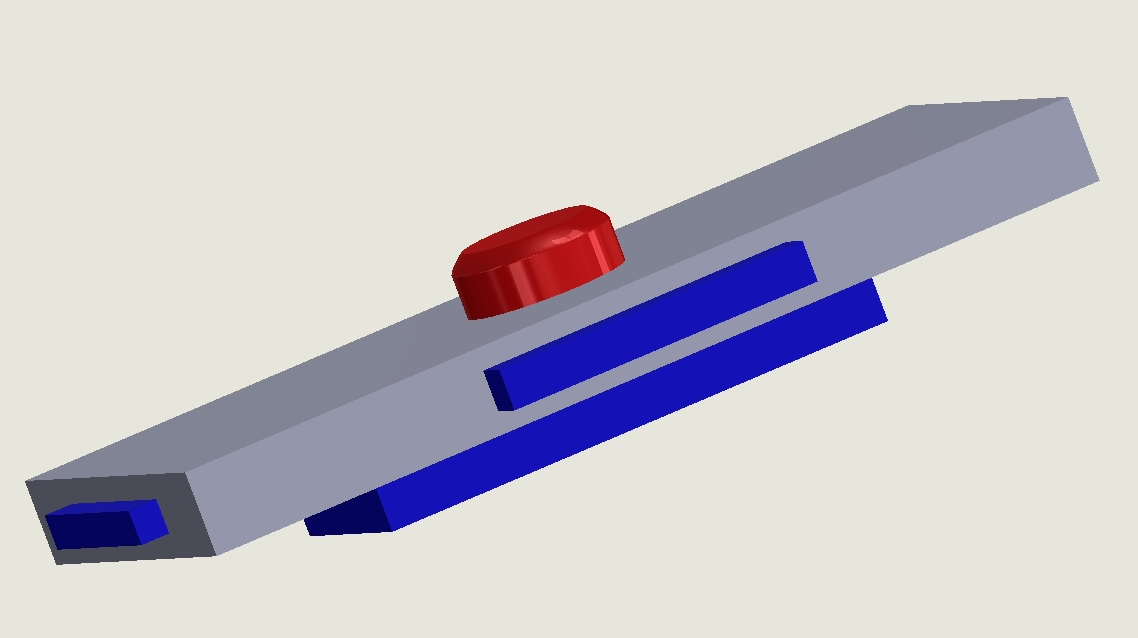
\includegraphics[width=0.8\textwidth]{Figures/Final.png}
  \caption{System Architecture}
  \label{fig:system_architecture}
\end{figure}

Where the microcontroller will be stored inside the box of the system and linked to the bluetooth module and the ultrasound sensors, which appear as blue boxes in Figure \ref{fig:system_architecture}, with the Gyroscope appearing with a Red Color.\\
The mounting of the circuit will be done as follows:
\begin{figure}[H]
  \centering

\tikzstyle{icdev}=[draw, text width=6em, minimum height=8em]

\begin{tikzpicture}[every node/.style = {font = \footnotesize},european]

    \node (digichip) [icdev,xshift=3cm,yshift=2cm] {};
    \draw (3.25,3.5) node(a1)[left]{$V_{cc}$};

    \draw (3.25,0.5) node(a2)[left]{GND};
    \draw (2.5,1.25) node(a3)[left]{PA4};
    \draw (2.5,1.75) node(a4)[left]{PA3};
    \draw (2.5,2.25) node(a5)[left]{PA2};
    \draw (2.5,2.75) node(a6)[left]{PA1};
    \draw (3.2,1.75) node(a7)[right]{OUT};
    \draw (6.5,1.75) node(a8)[rectangle]{HM-10};
    \draw (0.5,2.75) node(a9)[left]{VL53L1X};
    \draw (0.5,2.25) node(a10)[left]{VL53L1X};
    \draw (0.5,1.75) node(a11)[left]{VL53L1X};
    \draw (0.5,1.25) node(a12)[left]{MPU650};
    \draw (2.75,-0.5) node(a13)[ground]{};
    \draw (3,4.5) node(a14)[left]{};
    \draw (a13) -- (a2);
    \draw (a14) -- (a1);
    \draw (a3) -- (a12);
    \draw (a4) -- (a11);
    \draw (a5) -- (a10);
    \draw (a6) -- (a9);
    \draw (a7) -- (a8);

\end{tikzpicture}

  \caption{Microcontroller Circuit}
  \label{fig:system_architecture}
\end{figure}
Only the pins that are used in the circuit have been shown in the Figure.


\section{System Implementation}
\subsection{User Interface}
The user interface will be implemented using Python and the PyQt5 Library, which is a Python binding for the Qt5 GUI Library. The user interface will be composed of the following:
\begin{itemize}
  \item \textbf{Main Window:} The main window will be the first window that the user will see when the program is launched. It will contain the following:
  \begin{itemize}
    \item \textbf{Connect Button:} The connect button will be used to connect to the microcontroller via Bluetooth.
    \item \textbf{Disconnect Button:} The disconnect button will be used to disconnect from the microcontroller.
    \item \textbf{Start Button:} The start button will be used to start the data acquisition from the microcontroller.
    \item \textbf{Stop Button:} The stop button will be used to stop the data acquisition from the microcontroller.
    \item \textbf{Exit Button:} The exit button will be used to exit the program.
  \end{itemize}
  \item \textbf{Settings Window:} The settings window will be used to set the parameters for the data acquisition from the microcontroller. It will contain the following:
  \begin{itemize}
    \item \textbf{Start Button:} The start button will be used to start the data acquisition from the microcontroller.
    \item \textbf{Stop Button:} The stop button will be used to stop the data acquisition from the microcontroller.
    \item \textbf{Exit Button:} The exit button will be used to exit the program.
  \end{itemize}
  \item \textbf{Data Acquisition Window:} The data acquisition window will be used to display the data acquired from the microcontroller. It will contain the following:
  \begin{itemize}
    \item \textbf{Start Button:} The start button will be used to start the data acquisition from the microcontroller.
    \item \textbf{Stop Button:} The stop button will be used to stop the data acquisition from the microcontroller.
    \item \textbf{Exit Button:} The exit button will be used to exit the program.
  \end{itemize}
\end{itemize}

The user will be able to input a range for each parameter, or chose to ignore some of them, or even all of them in case of simple visualization of the data. If any system computed variable during any instant $t$ is not within the range specific by the user, it will trigger a response of LEDs and Sound Emitters which will signal that the quadcopter is not functioning as desired.

\subsection{Calculations and Measurements}
The microcontroller will be responsible for taking the measurements from the sensors and performing the necessary calculations and sending the results to the user interface. The microcontroller will be responsible for the following:

\begin{itemize}
  \item \textbf{Distance Measurement:} The distance measurement will be straightforward, the microcontroller will be automatically given the distance between the sensor and the object in front of it with the time of flight of the ultrasound signal.
  \item \textbf{Velocity Measurement:} The velocity measurement will be done point by point to be able to draw a graph of the velocity across each axis. The velocity will be calculated straightforwadly by the taking the distance $\Delta d$ at a time $t_i$ between points $i-1$ and $i$ and dividing it by the time interval between two sent iterations.
    \begin{equation}
      v_i = \frac{\Delta d}{\Delta t}
    \end{equation}  
  \item \textbf{Acceleration Measurement:} The acceleration measurement will be done point by point to be able to draw a graph of the acceleration across each axis. The acceleration will be calculated straightforwadly by the taking the velocity $\Delta v$ at a time $t_i$between points $i-1$ and $i$ and dividing it by the time interval between two sent iterations.
    \begin{equation}
      a_i = \frac{\Delta v}{\Delta t}
    \end{equation}
  \item \textbf{Orientation Measurement:} The measurement of the orientation is a bit more complex, but by using a Gyroscope, we could be comparing the inclination of the quadcopter with a base value then calculate the error and send it to the user interface.
\end{itemize}

\subsection{Control System}
The emission of the hyper-sound waves will be controlled via a Discrete Proportional Controller, which is a simple controller that is used to control the frequency of the sound waves emitted by the sound emitters. The controller will be designed as follows:
\begin{equation}
  u(n) = K_p e(n)
\end{equation}
Where $u(n)$ is the control signal, $K_p$ is the proportional gain, and $e(n)$ is the error signal \cite{Oppenheim2013Discrete}. The error signal will be calculated as follows:
\begin{equation}
  e(n) = r(n) - y(n)
\end{equation}
Where $r(n)$ is the reference signal, and $y(n)$ is the output signal. The reference signal will be the desired frequency of the sound waves, and the output signal will be the frequency of the sound waves emitted by the sound emitters. The controller will be implemented in the microcontroller, and the microcontroller will be responsible for sending the control signal to the sound emitters.
\tikzstyle{block} = [draw, fill=white, rectangle, 
    minimum height=3em, minimum width=6em]
\tikzstyle{sum} = [draw, fill=white, circle, node distance=1cm]
\tikzstyle{input} = [coordinate]
\tikzstyle{output} = [coordinate]
\tikzstyle{pinstyle} = [pin edge={to-,thin,black}]

\begin{figure}[H]
  \centering
 \begin{tikzpicture}[auto, node distance=2cm,>=latex']

    \node [input, name=input] {};
    \node [sum, right of=input] (sum) {-};
    \node [block, right of=sum] (controller) {Controller};
    \node [block, right of=controller, pin={[pinstyle]},
            node distance=3cm] (system) {System};

    \draw [->] (controller) -- node[name=u] {$u$} (system);
    \node [output, right of=system] (output) {};
    %\node [block, below of=u] (measurements) {Measurements};
    \coordinate [below of=u] (measurements) {};

    \draw [draw,->] (input) -- node {$r$} (sum);
    \draw [->] (sum) -- node {$e$} (controller);
    \draw [->] (system) -- node [name=y] {$y$}(output);
    %\draw [->] (y) |- (measurements);
    \draw [-] (y) |- (measurements);
    %\draw [->] (measurements) -| node[pos=0.99] {$-$} 
    \draw [->] (measurements) -| %node[pos=1.00] {$-$} 
        node [near end] {$y$} (sum);
        
    %\draw [->] 
  \end{tikzpicture}
  \caption{Block Diagram of the Control System}
\end{figure}
The controller is planned to be completed before the next phase of the project.




\tikzstyle{startstop} = [rectangle, rounded corners, 
minimum width=3cm, 
minimum height=1cm,
text centered, 
draw=black]
\tikzstyle{io} = [trapezium, 
trapezium stretches=true, % A later addition
trapezium left angle=70, 
trapezium right angle=110, 
minimum width=3cm, 
minimum height=1cm, text centered, 
draw=black]

\tikzstyle{process} = [rectangle, 
minimum width=4cm, 
minimum height=1cm, 
text centered, 
text width=3cm, 
draw=black]

\tikzstyle{decision} = [diamond, 
minimum width=2cm, 
minimum height=0.5mm,
text width= 8em, 
text centered, 
draw=black]
\tikzstyle{arrow} = [thick,->,>=stealth]
\subsection{Flowchart}
\begin{figure}[H]
\scalebox{0.8}[0.8]{
  \begin{tikzpicture}
    
    
      
    \node (start) [startstop] {Start};
  
    \node (p1) [process, below of=start, yshift=-1cm] {Input of the desired ranges of parameters of interest};
    \node (p2) [process, below of=p1, yshift= -1.5cm]{Signals are sent in predefined intervals};
    \node (p3) [process, below of=p2, yshift= -6.5cm]{The signals are then processed};
    \node (p4) [decision, below of=p3, yshift=-3.5cm]{Is W=0};
    \node (p5) [decision, below of=p4, xshift=-3cm, yshift=-2.5cm]{Is $S_{p} \notin R_{u} $};
    \node (p6) [process, below of=p5, yshift=-3cm]{W=1};
    \node (p7) [process, left of=p5, xshift=-4.5cm]{Do nothing};
    \node (p8) [startstop, left of=start, xshift=-2.5cm]{User end};
    \node (p9) [decision, below of=p4,xshift=3.5cm, yshift=-2.5cm]{Is $S_{p} \in R_{u} $};
    \node (p10) [process, below of=p9, yshift=-3cm]{W=0};
    \node (p11) [process, left of= p9,xshift=6cm]{Do nothing};
    \node (p12) [right of=p3, xshift=3cm]{};
    \node (p13) [right of= p2, xshift=3cm]{};
    \node (p14) [decision, below of=p2, yshift=-2.5cm]{Did the user input stop?};
    \node (p15) [process, left of =p3, xshift= -3.5cm]{Send parameters to the interface };
    \node (p16) [process, left of =p15, xshift= -3.5cm]{Display parameters on the interface};
    \draw [arrow] (start) -- (p1);
    \draw [arrow] (p1) -- (p2);
    \draw [arrow] (p2) -- (p14);
    \draw [arrow] (p3) -- (p4);
    \draw [arrow] (p4) -- node[anchor=east] {yes} (p5);
    \draw [arrow] (p5) -- node[anchor=east] {yes} (p6);
    \draw [arrow] (p5) -- node[anchor=north] {no} (p7);
    \draw [arrow] (p4) -- node[anchor=west] {no} (p9);
    \draw [arrow] (p9) -- node[anchor=east] {yes} (p10);
    \draw [arrow] (p9) -- node[anchor=north] {no} (p11);
    \draw [arrow] (p10) -| (p4);
    \draw [arrow] (p6) -|(p4);
    \draw (p3) -- (p12);
    \draw (p12) -- (p13);
    \draw [arrow] (p13) -- (p2);
    \draw [arrow] (p14) -| node[anchor=north] {yes} (p8);
    \draw [arrow] (p13) -- (p2);
    \draw [arrow] (p14) --node[anchor=west] {no} (p3);
    \draw [arrow] (p3) -- (p15);
    \draw [arrow] (p15) -- (p16);


  \end{tikzpicture}

}

  \caption{Algorithm of the system}
\end{figure}


\section{Kalman Filter}
The Kalman Filter is a state estimation algorithm that is used to estimate the state of a system given a set of measurements. It is used in a wide variety of applications such as robotics, navigation, and control. The Kalman Filter is a recursive algorithm that uses the previous state and the current measurement to estimate the current state. The Kalman Filter is composed of two parts, the prediction step and the update step.\cite{Kim2011Kalman} 
\subsection{Prediction Step}
The prediction step is used to predict the state of the system at the next time step. It is composed of the following:
\begin{itemize}
  \item \textbf{State Prediction:} The state prediction is used to predict the state of the system at the next time step. It is calculated by using the following equation:
    \begin{equation}
      \hat{x}_{k+1} = A\hat{x}_k + B u_k
    \end{equation}
  \item \textbf{Covariance Prediction:} The covariance prediction is used to predict the covariance of the system at the next time step. It is calculated by using the following equation:
    \begin{equation}
      P_{k+1} = A P_k A^T + Q
    \end{equation}
\end{itemize}
\subsection{Update Step}
The update step is used to update the state of the system at the current time step. It is composed of the following:
\begin{itemize}
  \item \textbf{Kalman Gain:} The Kalman Gain is used to calculate the optimal weighting between the prediction and the measurement. It is calculated by using the following equation:
    \begin{equation}
      K_k = P_{k+1} H^T (H P_{k+1} H^T + R)^{-1}
    \end{equation}
  \item \textbf{State Update:} The state update is used to update the state of the system at the current time step. It is calculated by using the following equation:
    \begin{equation}
      \hat{x}_k = \hat{x}_{k+1} + K_k (z_k - H \hat{x}_{k+1})
    \end{equation}
  \item \textbf{Covariance Update:} The covariance update is used to update the covariance of the system at the current time step. It is calculated by using the following equation:
    \begin{equation}
      P_k = (I - K_k H) P_{k+1}
    \end{equation}
\end{itemize}

We will be using the Kalman Filter to minimize the error in the measurements of the sensors. The Kalman Filter will be used to estimate the state of the system at each time step. The state of the system will be the position of the quadcopter in the 3D space. The measurements will be the distance measurements from the sensors and the orientation of the quadcopter.

The Kalman Filter is planned to be completed before the end of the next Phase.

\section{Conclusion and Future Work}
  The theoretical part of the project is still ongoing, but as it makes up the bulk of the project, and it will offer us a fruitful learning experience concerning both Kalman Filters and Discrete Time Control Systems, it is expected that the physical implementation of the project will start by the 10th of March, and will mostly be completed in a fraction of the time it takes to complete the theoretical study and algorithm of the system.\\
  We are expecting to abide by the following schedule.
  \begin{table}[H]
    \begin{tabular}{c|c}
      \textbf{Dates} & \textbf{Tasks} \\
      \midrule
      27 Feb. - 2 March & Theoretical study of the Kalman Filter \\
      3 March - 5 March & Theoretical study of Proportional Discrete time Control Systems  \\
      6 March - 9 March & Implementation of the various algorithms in C.\\
      10 March - 13 March & Creation of the User Interface and system Integration. \\
      13 March - 2 April & Testing and Debugging + Improvement of the System. \\
      \bottomrule
    \end{tabular}
  \end{table}
  And it leaves us enough time to abide by the project deliverabes in the following weeks.
  Now all that is left is the bibliography section

  \pagebreak
\bibliography{bibfile.bib}
\addcontentsline{toc}{section}{References}
\bibliographystyle{plain}
\nocite{*}


\end{document}
